\chapter{Zusammenfassung}\label{ch:zusammenfassung}

Im Rahmen einer Projektbearbeitung im Sommersemester 2020 wurde ein Framework für Couchbase erstellt, welches das bestehende Realm-Framework in der OUTPUT.DD App ersetzen sollte. Bei der Erstellung wurden im Rahmen eines Audits zahlreiche, teils strukturelle oder architekturelle, Probleme und Antipatterns in der bestehenden OUTPUT.DD App identifiziert. Die Problemstellung dieser Arbeit war es somit, nicht nur das neue Datenbank-Framework in der OUTPUT.DD App zu integrieren, sondern auch einen allumfassenden Neuaufbau zu planen und durchzuführen. Hierdurch sollten die identifizierten Probleme behoben und verschiedene Strategien entworfen werden, mit denen das Wiedereintreten dieser Probleme verhindert werden soll.

\section{Vorgehensweise und Ergebnisse}

\noindent Hierzu wurden verschiedene Software-Patterns beschrieben, sowie deren Anwendungsbereiche und weshalb deren Nutzung einen signifikanten Vorteil für die Separabilität, Funktionalität und Erweiterbarkeit als zentrale Bestandteile der Codequalität bietet. Außerdem wurde die Struktur der bestehenden App anhand einer Dialoglandkarte analysiert und anschließend, mit Hinblick auf die Struktur des neuen Couchbase-Frameworks, in eine neue Top-Level-Architektur überführt, die eine Separation der unterschiedlichen Komponenten vorschlägt. Mithilfe konkreter Konzepte für die Strukturierung von Verzeichnissen anhand der horizontalen und vertikalen Teilung wurde die Neuimplementierung der iOS-App konzipiert und durchgeführt. Hierbei wurde als statisches Code-Analysetool SwiftLint eingeführt, welches zur Vermeidung von Code Smells beitragen soll. Begonnen wurde mit der Neuimplementation des Frontends auf Grundlage einer Modularisierung und Wiederverwendung von UI-Komponenten, sowie der Orientierung an Prinzipien der Usability und der OUTPUT.DD Corporate Identity. Hierbei wurden unter gemeinsamer Absprache bestimmte Teile der App auch optisch modernisiert und durch ein Dark-Mode-Feature ergänzt. Um den redundanten Arbeitsaufwand bei der Übermittlung der iOS-Applikation an App Store Connect zu reduzieren und gleichzeitig die iOS-Applikation über TestFlight testen zu können, wurde eine CI-Pipeline konzipiert, dokumentiert und auf GitHub integriert.

\begin{figure}[H]
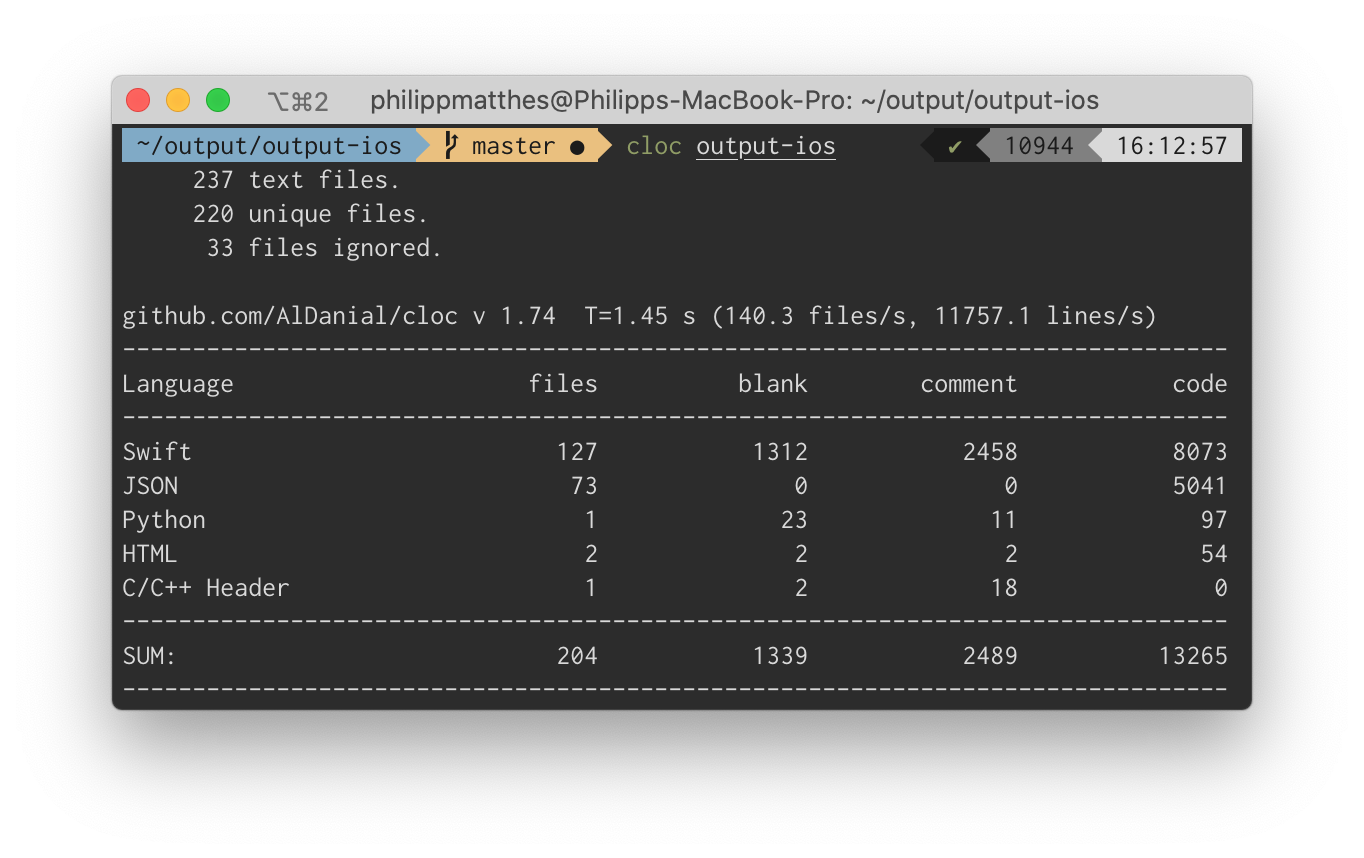
\includegraphics[width=\linewidth]{code.png}
\caption{Die neu implementierte App umfasst ca. 8000 Zeilen Swift Code.}\label{fig:code}
\end{figure}

\noindent Für die Integration des Datenbank-Backends wurden konkrete Patterns ausgewählt und verwendet, um gleichzeitig die Persistierung der Datenbankmodelle auf simulierten oder physischen Geräten und eine performante SwiftUI-Preview zu ermöglichen. Hierfür wurden insbesondere das Coordinator-Pattern, das Environment-Pattern, sowie das Proxy-Pattern verwendet. Durch die konsistente Nutzung dieser Architekturpattern konnte die Geschäftslogik der einzelnen Ansichten weiter voneinander separiert werden. Außerdem konnten die genannten Pattern genutzt werden, um zusätzlich zur lokalen Datenbank auch die Synchronisationskomponenten an diese anzubinden. Zum Testen der Datenbank- und Synchronisationsfunktionalitäten wurden konkrete Teststrategien angewandt, darunter die Generierung und Initialisierung von Daten zum Testen der Darstellung innerhalb der UI-Komponenten, sowie die Nutzung eines containerisierten Docker-Test-Setups für das Testen der Couchbase-Replikatoren. Abschließend wurden für die Implementation der Gamification-Errungenschaften konkrete Modelle und Basisalgorithmen entwickelt, mithilfe derer alle Errungenschaften weitestgehend unabhängig und separiert von den beteiligten UI-Komponenten implementiert werden konnten. Für die Fortführung des Projektes wurde diese Dokumentation neben weiteren Leitfäden mit besonders technischem Fokus erstellt, um als wesentlicher Teil des Entwicklerleitfadens zu dienen und zukünftig den Einstieg in die Entwicklung an der OUTPUT.DD App zu vereinfachen und zu vereinheitlichen.

\section{Offene Punkte}

Die Reimplementation der OUTPUT.DD App konnte vollständig durchgeführt werden und beinhaltet neben den bereits vorher existierenden Funktionalitäten, einer technischen, architekturellen und optischen Modernisierung auch allgemeine Verbesserungen in der Usability. Lediglich im Crowd-Monitoring-Framework konnten weitere Probleme identifiziert und kommuniziert werden, welche mithilfe klarer Integrationspunkte im Rahmen einer anderen Forschungsarbeit behoben werden sollen.

\noindent Bis zu OUTPUT.DD 2021 am 8. Juli 2021 wird die App weiterhin getestet und ggf. Verbesserungen und Optimierungen umgesetzt, welche sich aus dem Test-Feedback ergeben. Auch die Distribution der Apps und das Deployment des Couchbase-Backend auf einem Produktionssystem für OUTPUT.DD 2021 wird noch im Rahmen des Supportprozesses zukünftiger Teil dieser Arbeit sein.

\section{Danksagung}

Die Teilnahme an dieser Projektarbeit hat mir persönlich sehr viel Spaß gemacht und ich konnte meine Kenntnisse im Bereich Application Development weiter ausbauen. Ich danke meinem Betreuer, Dr. Thomas Springer, für das Vertrauen in meine Kompetenzen, mich mit einem sehr komplexen und vielseitigen Projekt wie diesem zu betrauen. Außerdem möchte ich B.Sc. Felix Kästner danken für die sehr kompetente Unterstützung bei der Implementation und Lösungsfindung auf Android-Seite.
